\chapter{Implementation Experiment}
\section{BSIL and TCL}
\subsection{Implementation} 

We implemented semi-symbolic model-checkers of BSIL and TCL with {\bf REDLIB} 
\cite{Wang03,Wang08a,Wang08b,Wang13,Wang14}
which is a free library for symbolic model-checking based on decision diagrams. 
{\bf REDLIB} supports symbolic pre-condition and post-condition calculation of discrete transitions.  
Our model-checker starts from a symbolic representataion of the initial condition. 
Then it repeatedly applies the post-condition procedure of {\bf REDLIB} to explore the symbolic state representations in the computation tree.
Our model-checker use the result in section~\ref{sec.mck.psp} to bound the exploration depth of tree.   

\subsection{Benchmarks and their experiment report} 

Then we experimented with two parameterized benchmarks.  
The first is the prisoners' dilemma described in Example~\ref{exmp.pd} with the number of prisoners as a parameter.
Then we applied the model-checker to check whether the model satisfies formula (A) and (B) in the introduction.
The time and memory usage of the model-checker is reported in Table~\ref{tab.exp.pd}.
\begin{table*}[!th]
\caption{Experiment data for the prisoners' dilemma model}
\label{tab.exp.pd}
\begin{center}
\begin{tabular}{c||c|c||c|c} \hline
\multirow{2}{*}{\#prisoners}  &\multicolumn{2}{c||}{Formula (A)} & \multicolumn{2}{c}{Formula (B)}\\ \cline{2-5}
& Time & Mem  & Time & Mem\\ \hline
2 &0.50s &72M   &0.51s &71M \\
3 &0.92s &75M   &0.88s &75M \\
4 &1.23s &83M   &1.14s &80M \\
5 &3.19s &146M  &2.90s &140M \\
6 &6.71s &388M  &6.52s &361M \\
7 &25.10s&1043M &23.11s&979M \\ \hline
\end{tabular}
\hspace*{10mm}
\parbox{50mm}{
s: seconds (computation time); \\
M: megabytes (memory usage); \\[2mm]
The experiment is conducted on a PC with Intel i7-2600k 3.4GHZ CPU 
and 8G RAM running Ubuntu 12.04. 
}
\end{center}
\end{table*}

The second benchmark is for campaign strategies 
of 2 political parties, Party $1$ and Party $2$, for seats in 
the congress.  
There are several parameters in our model, 
the number of seats in the congress, 
the amount of budget of each party in a round, 
and the number of candidates of each party in a round. 
The game is played by the chiefs of the parties, 
Chief $1$ (a gentleman) and Chief $2$ (a lady), 
who decide the amount of support that 
a candidate receive in a round.   
Candidates with more budget in a round will be elected in the round. 
If two or more candidates get the same amount of support, 
the winner will be decided randomly.  

In our model, in each round, chief 1 first decides his budget allotment, 
then chief 2 decides her budget allotment, and 
then the election result is determined.  
For example, with 3 dollars in his budget for two candidates, 
the strategy of a Chief can be written as 
$(x,y)\in\{(3,0), (2,1),(1,2),(0,3)\}$ where $x$ and $y$ 
respectively denote the support (in dollars) 
allotted to the first and the second candidates in his party. 
If Chief $1$ uses strategy $(2,1)$ and 
Chief $2$ uses strategy $(0,2)$ (Assume she has less budget.), 
the result of the round is 
that the two parties both win one seat in the round. 
On the other hand, if Chief $2$ chooses strategy $(1,1)$ instead, 
then there is no strategy for Chief $1$ to win more seats for his party. 

We use the following propositions and predicates to write 
specifications.  
For each $i\in[1,2]$ and $j\in[1,c]$ where $c$ is the number of 
candidates, 
$\textsl{elected}_{i,j}$ means the $j$'th candidate of party $i$ is 
elected now. 
Then we can use propositions $\textsl{elected}_{i,j}$ to construct 
a predicate $\textsl{win}_i$ that means party $i$ wins more seats than party $2-i$ in the round. 
Assume that the first candidate in each party is the chief. 
Then the following BSIL formula specifies that 
Chief $1$ has a strategy to make sure candidate 1 to be elected  
and in the same time allow the opponent party to win more seats in every round.
\begin{center} 
\hfill 
$\langle 1\rangle((\langle +\rangle\pevt \textsl{elected}_{1,1})
\wedge(\langle+2\rangle\pfrr \textsl{win}_2))$
\hfill (N) 
\end{center} 
Similarly, the following formula specifies that 
the chief of party 1 has a strategy to assure that his party 
can win more seats than his opponent party while allowing party two to assure 
the winning of a candidate.  
\begin{center} 
\hfill $\langle 1\rangle((\langle +\rangle \pevt \textsl{win}_1)
\wedge(\langle +2\rangle\pevt \textsl{elected}_{2,1}))$
\hfill (O)
\end{center} 
With different values of budget and candidate count, we may use our model-checker 
to analyze the strategy for achieving various goals.  
The time and memory usage data for checking formula (N) and (O) 
is in Table~\ref{tab.exp.vote}.
\begin{table*}[!th]
\caption{Experiment Data Election}
\label{tab.exp.vote}
\begin{center}
\begin{tabular}{c|c|c|c|c||c|c|c||c|c|c} \hline
\multicolumn{5}{c||}{Parameters}
&\multicolumn{3}{c||}{Formula (N)} 
& \multicolumn{3}{c}{Formula (O)}\\ \hline
$c_1$ & $b_1$ & $c_2$ & $b_2$ & $s$ & Result & Time & Mem & Result & Time & Mem\\ \hline
2&2 &2 &4 &1 &UNSAT &0.52s &61M  &UNSAT &0.53s &61M \\
2&4 &2 &4 &2 &UNSAT &1.20s &75M  &UNSAT &1.15s &75M \\
2&4 &2 &4 &3 &SAT   &0.73s &75M  &UNSAT &1.14s &75M \\
3&6 &3 &6 &3 &SAT   &1.51s &211M &UNSAT &0.93s &211M \\
3&9 &3 &6 &3 &UNSAT &9.14s &837M &SAT   &5.22s &681M \\
3&6 &3 &9 &3 &SAT   &8.74s &502M &UNSAT &8.49s &502M \\
3&9 &3 &9 &4 &SAT   &158s  &6631M&UNSAT &93.17s&5082M \\ \hline
\end{tabular}
\hspace*{2mm}
\parbox{75mm}{
$c_1$: \# candidates of party 1\\
$b_1$: total budget in a round of party 1\\
$c_1$: \# candidates of party 2\\
$b_1$: total budget in a round of party 2\\
$s$: \# of seats in the congress\\
}
\parbox{75mm}{
s: seconds (computation time)\\
M: megabytes (memory usage) \\[2mm]
The experiment is conducted on a PC with Intel i7-2600k 3.4GHZ CPU 
and 8G RAM running Ubuntu 12.04. 
}
\end{center}
\end{table*}

The experiment shows that some possibilities of using our tool to flexibly support the analysis and synthesis of collaborating strategies among several agents. 
In the experiment with the prisoners' dilemma, the prisoners are modelled as individual agents.  
In the experiment with the election game, the chairpersons of the parties are modelled as individual agents and their candidates and respective allocated budgets are modelled as numbers.  
It would be interesting to see how we can explore the techniques in modelling and specifying concurrent games with our tool.



As in the case of BSIL, we use the parametrised models of the iterated prisoners' dilemma 
as our benchmarks to check the performance of our implementation on TCL model checker.  
We use seven benchmark formulas on these models in our experiments.  
The first five benchmarks are taken from the examples (I) through (M) from the introduction.
Benchmarks (P) and (Q) are the following two properties, taken from \cite{WHY11}. 
\begin{list1} 
\item Property (P) specifies that all prisoners except Prisoner 1 can collaborate 
  to release Prisoner 1 and let Prisoner 1 decide their fate.

  $\langle 2,\ldots,m\rangle \big((\langle + \rangle \pevt \neg \mbox{\tt jail}_1) \wedge
  \bigwedge_{i \in \{2,\ldots m\}} (\langle +1 \rangle \pevt \neg \mbox{\tt jail}_i) \wedge
  (\langle +1 \rangle \pfrr \mbox{\tt jail}_i\big)$
  \hfill (P) 
\item Property (Q) specifies that Prisoner 1 has a strategy to put all other prisoners in jail while leaving her fate to them.

    $\langle 1\rangle \big( (\bigwedge_{i \in \{2,\ldots m\}} \langle + \rangle \pfrr \mbox{\tt jail}_i) \wedge
    (\langle 2,\ldots,m\rangle \pevt \neg \mbox{\tt jail}_1) \wedge \langle 2,\ldots,m\rangle \pfrr \mbox{\tt jail}_1 \big)$
  \hfill (Q) 
\end{list1} 
\begin{table*} 
\caption{Performance data of model-checking the TCL fragment}
\label{tab.perf}
\begin{center} 
\begin{tabular}{c||c|c|c|c|c|c|c|c|c} 
\hline 
\backslashbox{properties}{$m$}
& 2 & 3 & 4 & 5 & 6 & 7 & 8 & 9 & 10 \\ \hline \hline 
(I) 	
& 0.71s & 0.94s & 5.41s & 66.3s & 945s 	& \multicolumn{4}{c}{>1000s}\\ \cline{2-6} 
& 163M	& 165M 	& 185M 	& 350M	& 1307M	\\\hline 
(J) 
& 0.50s	& 0.52s	& 0.61s	& 0.71s & 1.11s	& 1.62s	& 5.77s & 20.9s	& 68.1s \\
  \cline{2-10} 
& 163M 	& 163M 	& 164M 	& 165M	& 168M	& 176M	& 214M	& 270M	& 376M	\\ \hline 
(K) 
& 0.51s	& 0.51s	& 0.6s	& 0.82s	& 1.01s	& 1.81s	& 5.54s	& 18.2s	& 48.3s	\\\cline{2-10} 
& 163M	& 163M	& 164M 	& 165M	& 168M	& 176M	& 200M	& 241M	& 318M	\\\hline 
(L) 
& 0.5s	& 0.51s	& 0.57s	& 0.74s	& 1.01s	& 1.79s	& 7.41s	& 33.8s	& 141s \\ \cline{2-10} 
& 163M	& 163M	& 164M	& 165M	& 168M	& 175M	& 232M	& 312M	& 430M \\\hline 
(M) 
& 0.51s	& 0.66s	& 19.1s & \multicolumn{6}{c}{>1000s} \\\cline{2-4} 
& 163M	& 164M	& 194M	\\\hline 
(P) 
& 0.51s	& 0.53s	& 0.61s	& 0.71s	& 1.01s	& 1.70s	& 5.38s	& 15.2s	& 53.7s	\\\cline{2-10} 
& 163M	& 163M	& 163M	& 165M 	& 168M	& 175M	& 202M	& 243M	& 295M	 \\\hline 
(Q) 
& 0.52s	& 0.52s	& 0.65s	& 0.72s	& 1.03s	& 1.85s	& 4.86s	& 16.1s	& 93.5s	 \\\cline{2-10} 
& 163M	& 163M	& 164M	& 165M	& 169M	& 177M	& 189M	& 208M	& 235M \\\hline 
\end{tabular} \\
s: seconds; 
M: megabytes. \\ 
The models are with 1 policeman and $m$ prisoners.
The experiment was carried out on an Intel i5 2.4G notebook 
with 2 cores and 4G memory, running ubuntu Linux version 11.10.  
\end{center} 
\end{table*} 
For these benchmarks, we have collected the performance data for various parameter values in Table~\ref{tab.perf}. 
For small models, the memory usage is dominated by the normal overhead, such as the representation of variable tables, state-transition tables, formula structures, etc. 
The data shows that our prototype can handle the various benchmarks, and scales well on five of the seven benchmarks.
Ignoring the overhead, it also shows the exponential growth.
The models, however, are growing exponentially, too.
We assume that this growth i the main cause of the exponential growth of the response time.

\section{Resilience}

\section{Tool implementation}
In the following, we report our implementation and experiment about checking a system's resilience to dense errors. 

We adopt {\em CEFSM} ({\em communicating extended finite-state machine})~\cite{BH89} as a convenient language for the description of abstract models of our concurrent game structures. 
A CEFSM consists of several finite-state machines extended with shared variables for the modeling of shared memory and with synchronizations for the modeling of message-passing in distributed systems.
This is justifiable since the fault-tolerant algorithms may themselves be subject to  
restrictions in concurrent or distributed computation.
Indeed, we found CEFSM very expressive in modeling the 
benchmarks from the literature \cite{CL99,RSB90}.  
\smallskip

The translation from our CEFSMs to state transition systems, 
such as finite Kripke structures, is standard in the literature. 
All state spaces, conditions, preconditions, post-conditions, 
fixed points, etc., are represented as logic formulas. 
The logic formulas are then implemented with multi-value decision diagrams 
(MDD) \cite{MD98}.  

We then took advantage of the support of REDLIB for writing down 
template automatas for constructing complex models. 
We specified a template automata with REDLIB to describe the moves of the players. 
Conceptually, the player automatas are constructed as an instance of the template automata. 
Then the whole game structure is constructed as the product of all player automatas. 
Finally, we use the API of REDLIB to do on-th-fly construction of the game structure which 
can be advantageous since unreachable states will never be generated.  

\subsection{Benchmarks and their experiment report}
We use the following five parameterized benchmarks to check the performance of our techniques. 
Each benchmark has parameters for the number of participating modules in the model.  
Such parameterized models come in handy for the evaluation of the scalability of our techniques with respect to concurrency and model sizes.  
\begin{itemize} 
\item[1.] We use the example of a fault-tolerant computer architecture 
  (Example~\ref{exmp.avi}) as our first benchmark.  
  An important feature of this benchmark is that there is an 
  assumed mechanism for detecting errors of the modules.  
  Once an error is detected, a processor can be assigned to recover the 
  module, albeit to the cost of a reduced redundancy in the executions.
\item[2.]
	Voting is a common technique for fault tolerance through 
  replication when there is no mechanism to detect errors of the 
  modules \cite{Pradhan96}.  
  In its simplest form, a system can guarantee correctness, provided less than half of its modules are faulty.   
  This benchmark implements this simple voting mechanism.  
  Every time a voting is requested, the modules submit their ballots individually.  
  Then we check how many module failures the system can endure and recover. 
\item[3.] This is a simplified version of the previous voting benchmark, where we assume that there is a blackboard 
  for the client to check the voting result.  
\item[4.] {\em Practical Byzantine fault-tolerance} ({\em PBFT}) algorithm: 
  We use an abstract model of the famous algorithm by 
  Castro and Liskov \cite{CL99}. 
  It does not assume the availability of an error-detection 
  mechanism but uses 
  voting techniques to guarantee the correctness of 
  computations when less than one third of the voters are faulty.  
  This algorithm has impact on the design of many protocols 
  \cite{AGGRW05,CMLRS06,KADCW09,GKVQ10,CWADM09} and is used in 
  Bitcoin \cite{bitcoin}, a peer-to-peer digital currency system.  
\item[5.] {\em Fault-tolerant clock synchronization algorithm}: 
  Clock synchronization is a central issue in distributed computing. 
  In \cite{RSB90}, 
  Ramanathan, Shin, and Butler presented 
  several fault-tolerance clock synchronization algorithms 
  in the presence of Byzantine faults with high probability.  
  We use a nondeterministic abstract model of the convergence averaging 
  algorithm from their paper.  
  The algorithm is proven correct when no more than one third of the 
  local clocks can drift to eight time units from the median of all clock 
  readings.  
\end{itemize}

\subsection{Modelling of the fault-tolerant systems}
Appropriate modelling of the benchmarks is always important for 
the efficient verification of real-world target systems. 
Many unnecessary details can burden the verification algorithm 
and blow up the computation, 
while sketchy models can then give too many false alarms 
and miss correct benchmarks.  
We have found that there is an interesting aspect 
in the modelling of the above benchmarks.  
Replication and voting are commonly adopted techniques for 
achieving fault-tolerance and resilience.  
Such fault-tolerant algorithms usually consist of 
several identical modules that use the same behavior templates.  
This observation implies that the identity of individual modules 
can be unimportant for some benchmarks.  
For such benchmarks, we can use counter abstraction 
\cite{ET99,Lubachevsky84} in their models.  
Specifically, with counter abstraction, 
we can model all system players with one player that keeps a counter $c(l)$ 
for each control location $l$ in the template automatas. 
Then at a state of the whole game graph, 
$c(l)$ records the number of system players at location $l$.  
With this technique, a system with $m-1$ system player and one error model player is 
then reduced to two players: one counter-abstraction player for all the system players and one 
remaining error model player. 
If a system player enters a location $l$ in a global transition, 
then in the model, $c(l)$ is incremented by one in the abstract global transition. 
If a system player leaves $l$ in the global transition, 
then $c(l)$ is decremented by one in the abstract global transition.  
But the succession of location movements of a particular player is omitted from the abstraction. 
 

We found that we can use counter abstraction to 
prove the correctness of benchmarks 1, 2, and 3. 
In contrast, the PBFT and the clock synchronization algorithms use 
counters for each module to model the responses received 
from its peer modules. 
As a result, we decided not to use counter abstraction to model 
these two algorithms in this work. 

In the following, we explain how to apply our techniques to analyze 
the resilience levels of the avionic systems 
in Example~\ref{exmp.avi}.  
The application is achieved in three steps.
We first model the system under analysis either as a plain CEFSM or with counter abstraction (if our analysis tool cannot handle the complexity of the plain CEFSM).
We then build the product automaton of the CEFSM as the resilience 
game structure except for the move vectors.  
Finally, we convert the labels on the transitions of the product automaton to 
move vectors of the two players. 
Note that the moves may not correspond to the transition labels of the CEFSM.  

\subsection*{Step 1: the construction of the CEFSM}
We first present the CEFSM model template 
of Example~\ref{exmp.avi} in Figure~\ref{fig.pm}. 
\begin{figure*}[t] 
\begin{center} 
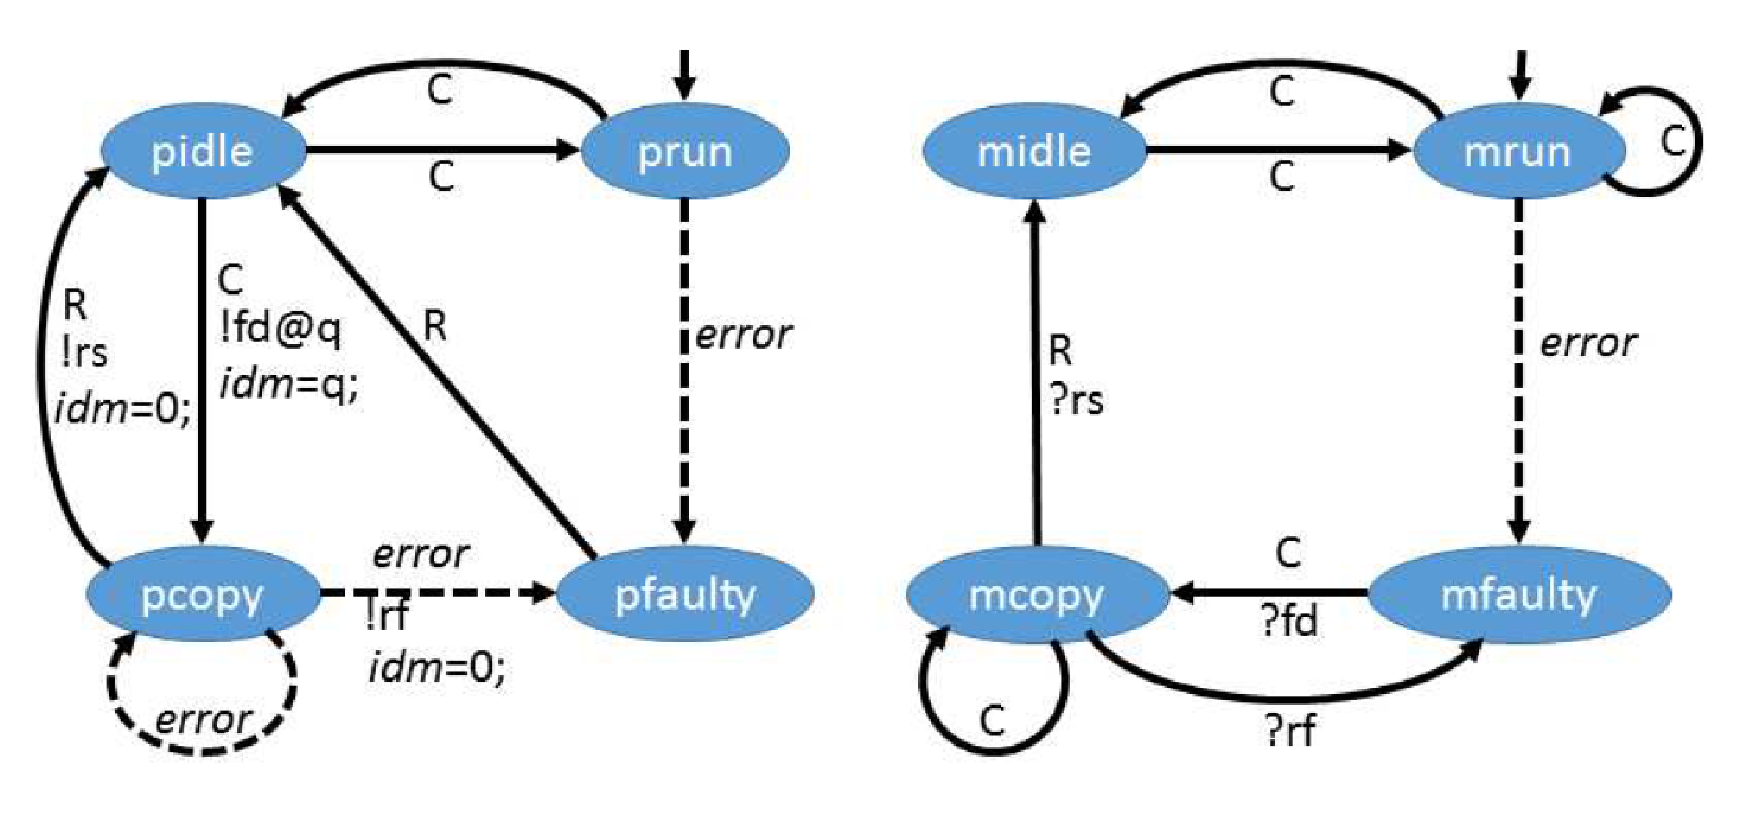
\epsfig{file=avi.eps,width=140mm} 
\caption{CEFSM templates of $n$ processors and $m$ memory copies}
\label{fig.pm}
\end{center} 
\end{figure*}
The CEFSM model has $n$ processors and $m$ memory modules. 
Figures~\ref{fig.pm}(a) and (b) are 
for the abstraction of processors and memory copies, respectively.  
The ovals represent local states of a processor or a 
memory module, while the arrows represent transitions. 
The transitions of a CEFSM are labeled with `$\emerr$', 
`C' (for Control), or `R' (for recovery).  

We also use synchronizers to bind process transitions. 
For example, when a memory module moves into a faulty state, 
an idle processor may issue an {\tt fd} (error-detected) event
and try to repair the module by copying memory contents from 
normal memory modules.  
Such error-detection is usually achieved with standard hardware.  
Note that the benchmarks are models that reflect the 
recovery mechanism, abstracting away the details of the original systems.  
A central issue in the design of this recovery mechanism is then 
the resilience level of the controlled systems.  
We need three synchronizers: 
\textit{fd} for error detection by a processor, 
\textit{rs} for recovery success, 
and \textit{rf} for recovery failure.  
The three synchronizers are used to bind a transition from a processor 
and another from a memory module into a synchronized transition.  
For example, a processor at state \textit{pidle} and 
a memory module at state 
\textit{mfaulty} may simultaneously enter their 
\textit{pcopy} and \textit{mcopy} states respectively
through synchronizers $!$\textit{fd} (for sending the synchronizer) 
and $?$\textit{fd} (for receiving). 
We also conveniently use a variable $q$ in this synchronized 
transition to capture the identifier of the memory module receiving 
the synchronizer.  
A transition without synchronization labels is considered a trivial 
synchronized transition.  
The transition system of the CEFSM operates with interleaving semantics 
at the abstraction level of the synchronized transitions. 

For counter abstraction, we need four global variables \textit{crp}, \textit{cfp}, 
\textit{crm}, and \textit{cfm} respectively 
to keep track of the numbers of running processors, faulty processors, 
running memory modules, and faulty memory modules. 
We also need a local variable \textit{idm} for each processor to record 
the faulty memory module identifier that the processor is 
responsible for recovery. 
We label the controllable, error, and recovery 
transitions respectively with `C', `$\emerr$', and `R'. 
We also label each transition with synchronizers and actions.  
At any moment, the processors and the memory modules 
may enter their running states, execute a task, and generate 
the outcome. 
A processor starts its execution from state \textit{prun} while 
a memory module starts from state \textit{mrun}. 


\subsection*{Step 2: building the product automata}
The product automata is a Kripke structure whose 
states are of is a vector $[p_1,\ldots,p_n,i_1,\ldots,i_n,s_1,\ldots,s_m]$ 
of $2n+m$ elements.  
For all $k$, $p_k$ and $i_k$ respectively represent the 
current location and the current \textit{idm} value of processor $k$ while 
$s_k$ represents the current location of memory module $k$.  
Then interleaving semantics that each time only a global transition 
(a single local process transition without synchronizers 
or two local process transition bound by a synchronizer) is executed 
is adopted to determine the transition relation from one state to another. 
Such techniques are standard in model construction.  
REDLIB can help in this regard by constructing the Kripke structure in 
an on-the-fly style to avoid the construction of those states not reachable 
from the initial state. 

\subsection*{Step 3: the labeling of the move vectors} 
After the second step, we have the game structure ready except for the 
move vectors on the transitions. 
We use $E_1=\{C,R,\mbox{\em nop}\}$, where {\em nop} represents ``no operation,"
and $E_2=\{\emnerr,\emerr\}$.  
Then we use the following three rules to label move vectors. 
\begin{list1} 
\item Every global transition with one component local process transition labeled 
	with $\emerr$ is labed with move vector $[\mbox{\em nop},\emerr\}$.  
\item Every global transition with a component local process transition labeled 
	with $R$ 	
	is labeled with move vector $[R,\emnerr]$.  
\item All other global transitions are labeled with move vector $[C,\emnerr]$.  
\end{list1} 


\subsection*{Counter abstraction of the example} 
We also use the CEFSM in figure~\ref{fig.pm} to explain counter abstraction. 
We need eight counter variables: 
{\em pr}, 
{\em pi}, 
{\em pc}, 
{\em pf}, 
{\em mr}, 
{\em mi}, 
{\em mc}, and 
{\em mf} to respectively record the 
number of processes in location prun, pidle, pcopy, pfaulty, mrun, midle, mcopy, and mfaulty
in a state.  
Then the counter abstraction of the CEFSM is in Figure~\ref{fig.pmC}.  
\begin{figure*}[t] 
\begin{center} 
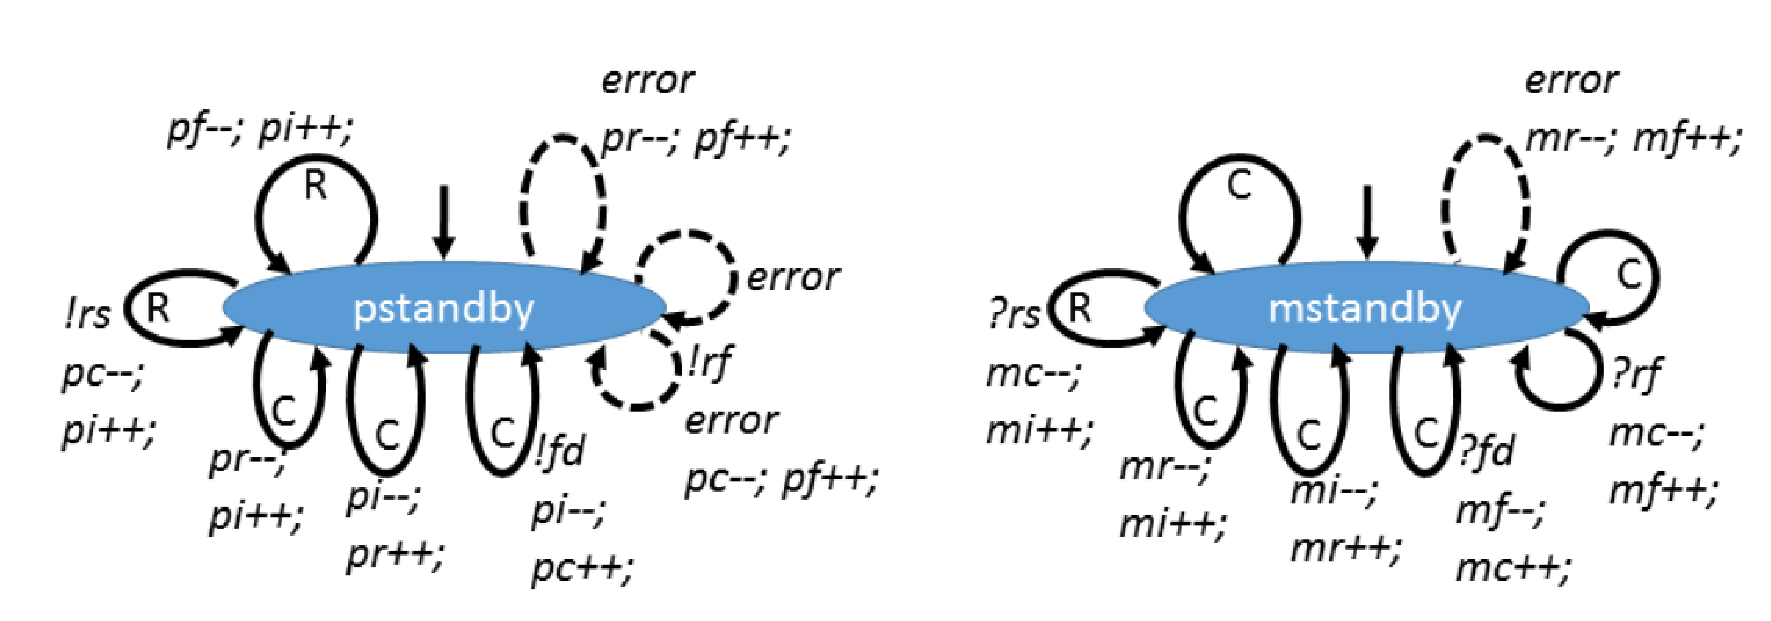
\epsfig{file=aviC.eps,width=140mm} 
\caption{Counter abstraction of the CEFSM templates of $n$ processors and $m$ memory copies}
\label{fig.pmC}
\end{center} 
\end{figure*}
The initial state are specified with constraint: 
$\mbox{\em pr}=n
\wedge \mbox{\em pi}=0
\wedge \mbox{\em pc}=0
\wedge \mbox{\em pf}=0
\wedge \mbox{\em mr}=m
\wedge \mbox{\em mi}=0
\wedge \mbox{\em mc}=0
\wedge \mbox{\em mf}=0$
on the counters.  
The state in the product automata must satisfy the following constraints: 
$\mbox{\em pr}+\mbox{\em pi}+\mbox{\em pc}+\mbox{\em pf}=n
\wedge \mbox{\em mr}+\mbox{\em mi}+\mbox{\em mc}+\mbox{\em mf}=m$.  
As can be seen, we do not care which processor is in the idle mode, 
in the running mode, etc., in this abstraction. 
Similarly, we do not care which memory module is in the idle mode, in the running mode, and etc. 
The local state transition only keeps tracks of the number of processors in each mode and 
the number of memory modules in each mode. 
We also do not care which processor is in charge of the recovery of which memory module.  
Such an abstraction can be done automatically.  

The labeling of the move vectors on the transitions in the Kripke structure (product automaton)
follows the same rules for the product automaton from the CEFSM in Figure~\ref{fig.pm}.  




\subsection*{Analysis of the game structure} 
The majority outcome of the processors and memory copies 
is used as the outcome of the system.  
A processor may enter the faulty state.  
A memory module may also enter the faulty state. 
Processors may control to recover themselves or a faulty memory module 
by copying the contents of a functioning memory module to 
the faulty one.  
At any moment, we want to make sure that we can always recover 
to a global condition with the following two restrictions. 
\begin{itemize} 
\item There are at least two more processors in \label{reply2.2more} 
	the running mode than the processors in the faulty mode.  
\item There are at least two more memory copies in 
	the running mode than memory copies in the faulty mode. 
\end{itemize} 
Together, the failure condition is 
$\textit{crp}-\textit{cfp}<2\vee\textit{crm}-\textit{cfm}<2$.  
That is, all states in the transition system satisfying 
$\textit{crp}-\textit{cfp}<2\vee\textit{crm}-\textit{cfm}<2$ 
are in set $F$.  

We report the performance data 
in Table~\ref{tab.perf} for the resilience algorithms 
described in Section~\ref{subsec.bench} 
against the parameterized benchmarks in the above with various 
parameters.  
The second column shows the concurrency sizes.  
The third column shows the values of $k$ for the rows.  
The fourth and fifth columns show the sizes of the concurrent game structures.  
The sixth and seventh columns show the time and spaces used to calculate 
sfrch$_k()$.  
Similarly, the eighth and ninth columns show the time and spaces for calculating 
the res$_k()$.  

The benchmark in Figure~\ref{fig.pm} does not have nodes in 
$\safe_2(G)$ and $\res_2(G)$.  
So we changed the benchmark to see how we check our implementation 
with $k>1$.  
The change is that the recovery transition from state \textit{pcopy} to 
\textit{pidle}
of processors are relabeled as controllable. 
This change significantly limits the ability of the system errors 
to derail the system.  
\begin{table*}[t] 
\caption{Performance data for resilience calculation \hspace{21mm} s: seconds; M: megabytes} 
\label{tab.perf} 
\begin{center} 
\resizebox{\columnwidth}{!}{
\begin{tabular}{l|c|c|c|c||c|c||c|c} \hline 
benchmarks & concurrency & $k$ & \multicolumn{2}{c||}{game sizes} 
& \multicolumn{2}{c||}{sfrch$_k$}  
			& \multicolumn{2}{c}{res$_k$} \\\cline{4-9} 
	 & 	& & \#nodes & \#edges & time  & memory   & time & memory  \\
\hline \hline 
avionics & 2 processors \& 2 memory modules 
     & 2 & 118 & 750 
     & 0.62s & 114M & 0.85s & 116M \\ \cline{2-9} 
     & 2 processors \& 3 memory modules 
     & 2 & 414 & 3252
     & 0.94s & 139M & 1.10s & 153M \\ \cline{2-9} 
     & 3 processors \& 3 memory modules 
     & 3 & 1540 & 15090 
     & 4.67s & 225M & 8.38s & 267M \\ \cline{2-9} 
     & 3 processors \& 4 memory mdules
     & 3 & 5601 & 63889 
     & 42.86s & 815M & 155s & 846M \\ \hline  
avionics & 6 processors \& 6 memory modules 
	 & 2 & 1372 & 6594 
	 & 2.89s & 129M & 3.54s & 516M \\ \cline{2-9} 
(counter	 & 7 processors \& 7 memory modules 
	 & 3 & 2304 & 11396 
	 & 10.7s & 216M & 23.4s & 808M \\ \cline{2-9}
abstraction)	 & 8 processors \& 8 memory modules 
	 & 3 & 3645 & 18432 
	 & 43.8s & 1009M & 135s & 2430M \\ \hline 
voting	 & 1 client \& 20 replicas 
	 & 9 & 9922 & 23551 & 7.01s & 260M & 36.7s & 297M \\ \cline{2-9} 
	 & 1 client \& 26 replicas 
	 & 12 & 20776 & 49882 & 19.9s & 474M & 79.6s & 611M \\ \hline 
simple	 & 1 client \& 150 replicas 
	 & 74 & 458 & 1056 & 0.71s & 159M & 31.7s & 219M \\ \cline{2-9} 
voting	 & 1 client \& 200 replicas 
	 & 99 & 608 & 1406 & 1.06s & 161M & 162s & 337M \\ \cline{2-9} 
	 & 1 client \& 250 replicas 
	 & 124 & 758 & 1756 & 1.36s & 163M & 307s & 499M \\ \hline 
PBFT 	 & 1 client \& 6 replicas 
	 & 2 & 577 & 897 & 0.34s & 72M & 1.05s & 193M \\ \cline{2-9} 
	 & 1 client \& 9 replicas 
	 & 4 & 2817 & 4609 & 13.3s & 564M & 58.5s & 1657M \\ \hline 
clock	 & 1 client \& 15 servers  
	 & 7 & 16384 & 229376 & 45.1s & 3075M & 62.4s & 3264M  \\ \cline{2-9} 
sync	 & 1 client \& 17 severs  
	 & 8 & 65536 & 1070421 & 870s & 14725M & 915s & 15433M  \\ \hline 
\end{tabular}
}
\end{center}
\vspace*{-5mm}
\end{table*}
For the avionics system, %the $k$ value
the resilience level $k$ is set to 
one less than half the %value
number of processors.  
For the voting and simple voting benchmarks, 
the value of $k$ is set to one less than half the number of 
replicas (voters). 
For the PBFT and clock synchronization algorithm, we choose 
$k$ to be one less than one third of the number of replicas. 

The performance data has been collected with a Virtual Machine (VM) 
running opensuse 11.4 x86 
on Intel i7 2600k 3.8GHz CPU 
with 4 cores and 8G memory. 
The VM only uses one core and 4G memory.  

The time and space used to calculate resilience is a little bit more 
than that to check for $\safe$.  
The reason is that $\safe_k$ is a pre-requisite for calculating $\res_k$.  
In our experiment, $\safe_k$ is usually 
very close to $\res_k$ and does not require much extra time in 
calculating $\res_k$ out of $\safe_k$.  

The experiments show that our techniques 
scale to realistic levels of redundancy.  
For fault-tolerant hardware, usually the numbers of replicas are small, 
for example, less than 10 replicas. 
Thus our techniques seem very promising for the 
verification and synthesis\label{reply2.verification.hardware} of hardware fault-tolerance.  

On the other hand, 
nowadays, software fault-tolerance through networked computers can 
create huge numbers of replicas.  
Our experiment shows that counter abstraction can be a useful 
techniques for the modeling and verification of software resilience.  
Specifically, for the avionics benchmark, 
we can verify models of much higher concurrency and complexity with 
counter abstraction than without. 
% As can be seen, our techniques can really prove the % safety and 
% resilience of pretty large concurrency sizes.  


